% GNUPLOT: LaTeX picture with Postscript
\begingroup
  \makeatletter
  \providecommand\color[2][]{%
    \GenericError{(gnuplot) \space\space\space\@spaces}{%
      Package color not loaded in conjunction with
      terminal option `colourtext'%
    }{See the gnuplot documentation for explanation.%
    }{Either use 'blacktext' in gnuplot or load the package
      color.sty in LaTeX.}%
    \renewcommand\color[2][]{}%
  }%
  \providecommand\includegraphics[2][]{%
    \GenericError{(gnuplot) \space\space\space\@spaces}{%
      Package graphicx or graphics not loaded%
    }{See the gnuplot documentation for explanation.%
    }{The gnuplot epslatex terminal needs graphicx.sty or graphics.sty.}%
    \renewcommand\includegraphics[2][]{}%
  }%
  \providecommand\rotatebox[2]{#2}%
  \@ifundefined{ifGPcolor}{%
    \newif\ifGPcolor
    \GPcolortrue
  }{}%
  \@ifundefined{ifGPblacktext}{%
    \newif\ifGPblacktext
    \GPblacktexttrue
  }{}%
  % define a \g@addto@macro without @ in the name:
  \let\gplgaddtomacro\g@addto@macro
  % define empty templates for all commands taking text:
  \gdef\gplbacktext{}%
  \gdef\gplfronttext{}%
  \makeatother
  \ifGPblacktext
    % no textcolor at all
    \def\colorrgb#1{}%
    \def\colorgray#1{}%
  \else
    % gray or color?
    \ifGPcolor
      \def\colorrgb#1{\color[rgb]{#1}}%
      \def\colorgray#1{\color[gray]{#1}}%
      \expandafter\def\csname LTw\endcsname{\color{white}}%
      \expandafter\def\csname LTb\endcsname{\color{black}}%
      \expandafter\def\csname LTa\endcsname{\color{black}}%
      \expandafter\def\csname LT0\endcsname{\color[rgb]{1,0,0}}%
      \expandafter\def\csname LT1\endcsname{\color[rgb]{0,1,0}}%
      \expandafter\def\csname LT2\endcsname{\color[rgb]{0,0,1}}%
      \expandafter\def\csname LT3\endcsname{\color[rgb]{1,0,1}}%
      \expandafter\def\csname LT4\endcsname{\color[rgb]{0,1,1}}%
      \expandafter\def\csname LT5\endcsname{\color[rgb]{1,1,0}}%
      \expandafter\def\csname LT6\endcsname{\color[rgb]{0,0,0}}%
      \expandafter\def\csname LT7\endcsname{\color[rgb]{1,0.3,0}}%
      \expandafter\def\csname LT8\endcsname{\color[rgb]{0.5,0.5,0.5}}%
    \else
      % gray
      \def\colorrgb#1{\color{black}}%
      \def\colorgray#1{\color[gray]{#1}}%
      \expandafter\def\csname LTw\endcsname{\color{white}}%
      \expandafter\def\csname LTb\endcsname{\color{black}}%
      \expandafter\def\csname LTa\endcsname{\color{black}}%
      \expandafter\def\csname LT0\endcsname{\color{black}}%
      \expandafter\def\csname LT1\endcsname{\color{black}}%
      \expandafter\def\csname LT2\endcsname{\color{black}}%
      \expandafter\def\csname LT3\endcsname{\color{black}}%
      \expandafter\def\csname LT4\endcsname{\color{black}}%
      \expandafter\def\csname LT5\endcsname{\color{black}}%
      \expandafter\def\csname LT6\endcsname{\color{black}}%
      \expandafter\def\csname LT7\endcsname{\color{black}}%
      \expandafter\def\csname LT8\endcsname{\color{black}}%
    \fi
  \fi
    \setlength{\unitlength}{0.0500bp}%
    \ifx\gptboxheight\undefined%
      \newlength{\gptboxheight}%
      \newlength{\gptboxwidth}%
      \newsavebox{\gptboxtext}%
    \fi%
    \setlength{\fboxrule}{0.5pt}%
    \setlength{\fboxsep}{1pt}%
    \definecolor{tbcol}{rgb}{1,1,1}%
\begin{picture}(9060.00,4520.00)%
    \gplgaddtomacro\gplbacktext{%
      \csname LTb\endcsname%%
      \put(444,450){\makebox(0,0)[r]{\strut{}$0$}}%
      \csname LTb\endcsname%%
      \put(444,855){\makebox(0,0)[r]{\strut{}$2$}}%
      \csname LTb\endcsname%%
      \put(444,1260){\makebox(0,0)[r]{\strut{}$4$}}%
      \csname LTb\endcsname%%
      \put(444,1665){\makebox(0,0)[r]{\strut{}$6$}}%
      \csname LTb\endcsname%%
      \put(444,2070){\makebox(0,0)[r]{\strut{}$8$}}%
      \csname LTb\endcsname%%
      \put(444,2475){\makebox(0,0)[r]{\strut{}$10$}}%
      \csname LTb\endcsname%%
      \put(444,2879){\makebox(0,0)[r]{\strut{}$12$}}%
      \csname LTb\endcsname%%
      \put(444,3284){\makebox(0,0)[r]{\strut{}$14$}}%
      \csname LTb\endcsname%%
      \put(444,3689){\makebox(0,0)[r]{\strut{}$16$}}%
      \csname LTb\endcsname%%
      \put(444,4094){\makebox(0,0)[r]{\strut{}$18$}}%
      \csname LTb\endcsname%%
      \put(444,4499){\makebox(0,0)[r]{\strut{}$20$}}%
      \csname LTb\endcsname%%
      \put(542,274){\makebox(0,0){\strut{}$0$}}%
      \csname LTb\endcsname%%
      \put(1374,274){\makebox(0,0){\strut{}$2$}}%
      \csname LTb\endcsname%%
      \put(2205,274){\makebox(0,0){\strut{}$4$}}%
      \csname LTb\endcsname%%
      \put(3037,274){\makebox(0,0){\strut{}$6$}}%
      \csname LTb\endcsname%%
      \put(3869,274){\makebox(0,0){\strut{}$8$}}%
      \csname LTb\endcsname%%
      \put(4700,274){\makebox(0,0){\strut{}$10$}}%
    }%
    \gplgaddtomacro\gplfronttext{%
      \csname LTb\endcsname%%
      \put(3736,4068){\makebox(0,0)[r]{\strut{}CC2}}%
      \csname LTb\endcsname%%
      \put(3736,3892){\makebox(0,0)[r]{\strut{}CCSD}}%
      \csname LTb\endcsname%%
      \put(3736,3716){\makebox(0,0)[r]{\strut{}HF}}%
      \csname LTb\endcsname%%
      \put(87,2474){\rotatebox{-270.00}{\makebox(0,0){\strut{}X sec  (a.u.)}}}%
      \csname LTb\endcsname%%
      \put(2621,10){\makebox(0,0){\strut{}$\mathrm{E_I+E_k}$ (eV)}}%
    }%
    \gplgaddtomacro\gplbacktext{%
      \csname LTb\endcsname%%
      \put(4783,450){\makebox(0,0)[r]{\strut{}}}%
      \csname LTb\endcsname%%
      \put(4783,855){\makebox(0,0)[r]{\strut{}}}%
      \csname LTb\endcsname%%
      \put(4783,1260){\makebox(0,0)[r]{\strut{}}}%
      \csname LTb\endcsname%%
      \put(4783,1665){\makebox(0,0)[r]{\strut{}}}%
      \csname LTb\endcsname%%
      \put(4783,2070){\makebox(0,0)[r]{\strut{}}}%
      \csname LTb\endcsname%%
      \put(4783,2475){\makebox(0,0)[r]{\strut{}}}%
      \csname LTb\endcsname%%
      \put(4783,2879){\makebox(0,0)[r]{\strut{}}}%
      \csname LTb\endcsname%%
      \put(4783,3284){\makebox(0,0)[r]{\strut{}}}%
      \csname LTb\endcsname%%
      \put(4783,3689){\makebox(0,0)[r]{\strut{}}}%
      \csname LTb\endcsname%%
      \put(4783,4094){\makebox(0,0)[r]{\strut{}}}%
      \csname LTb\endcsname%%
      \put(4783,4499){\makebox(0,0)[r]{\strut{}}}%
      \csname LTb\endcsname%%
      \put(4881,274){\makebox(0,0){\strut{}$0$}}%
      \csname LTb\endcsname%%
      \put(5921,274){\makebox(0,0){\strut{}$0.5$}}%
      \csname LTb\endcsname%%
      \put(6960,274){\makebox(0,0){\strut{}$1$}}%
      \csname LTb\endcsname%%
      \put(8000,274){\makebox(0,0){\strut{}$1.5$}}%
      \csname LTb\endcsname%%
      \put(9039,274){\makebox(0,0){\strut{}$2$}}%
    }%
    \gplgaddtomacro\gplfronttext{%
      \csname LTb\endcsname%%
      \put(8075,4068){\makebox(0,0)[r]{\strut{}CC2}}%
      \csname LTb\endcsname%%
      \put(8075,3892){\makebox(0,0)[r]{\strut{}CCSD}}%
      \csname LTb\endcsname%%
      \put(8075,3716){\makebox(0,0)[r]{\strut{}HF}}%
      \csname LTb\endcsname%%
      \put(6960,10){\makebox(0,0){\strut{}$\mathrm{E_I+E_k}$ (eV)}}%
    }%
    \gplbacktext
    \put(0,0){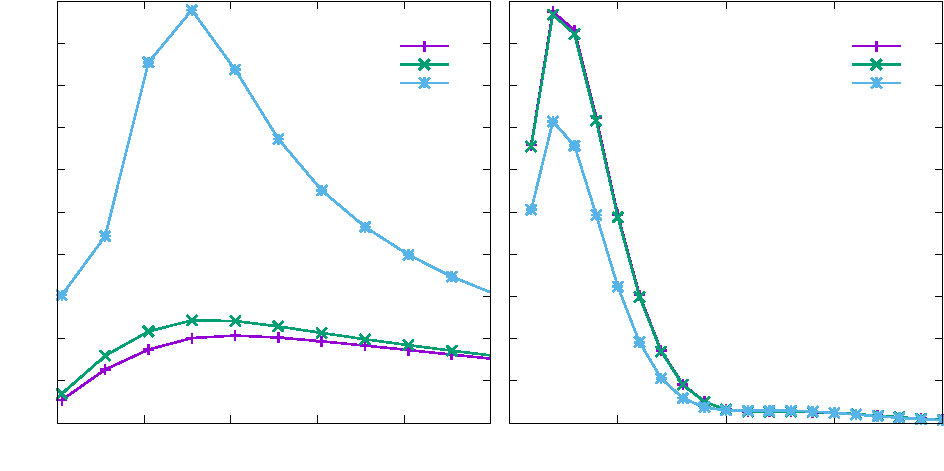
\includegraphics[width={453.00bp},height={226.00bp}]{chapters/results/image/ezDyson}}%
    \put(1100,1200){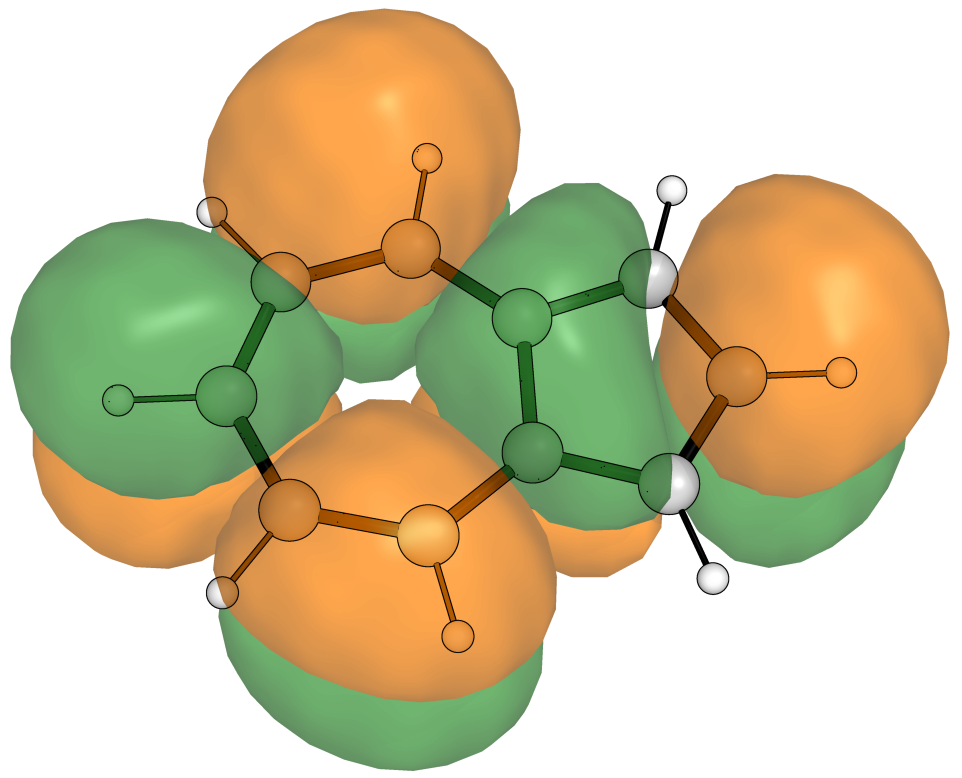
\includegraphics[scale=0.45]{chapters/results/image/azulene.png}}%
    \put(6300,1100){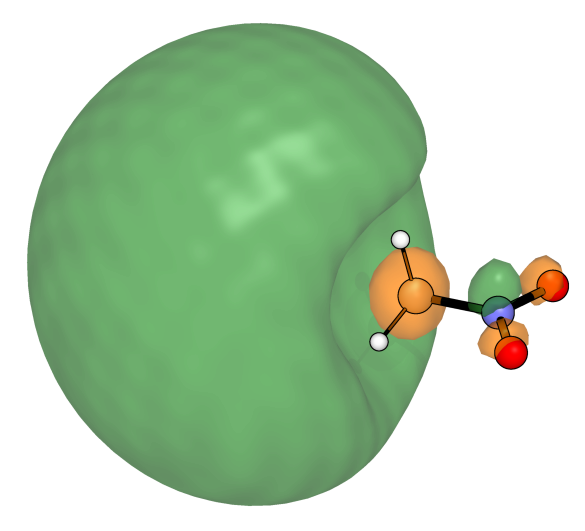
\includegraphics[scale=0.7]{chapters/results/image/MeNO2_DBS.png}}%
    \gplfronttext
  \end{picture}%
\endgroup
